\problemname{Xortris}

\illustration{.3}{xorworld}{Screenshot of World of Xor}

It is 1990 and you are in the development team of a video game that is
going to revolutionize the future of arcades. The player is given a
rectangular board with some white and black squares. The goal is to
turn the whole board white. At each turn, the player may choose a
tetromino from an infinite supply, move and rotate it within the
limits of the board, and toggle the colour of the four squares covered by
the tetromino. A tetromino is a connected set of 4 squares (see
Figure~\ref{fig:tetrominoes}).

Unfortunately, the testing team has been complaining about some levels
being impossible to solve. You know that testers are skilled enough to
place a piece in any position and rotation needed, so the problem may
be somewhere else. Your next debugging step is to write a program that
checks whether a level is solvable.

\begin{figure}[h]
  \centering
  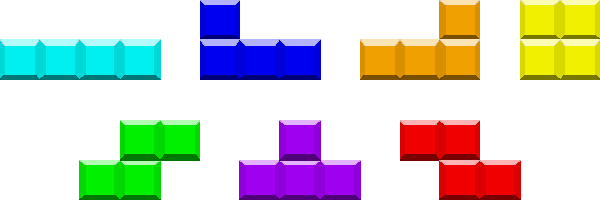
\includegraphics[width=0.5\textwidth]{Tetrominoes_IJLO_STZ_Worlds}
  \caption{All tetrominoes.
  \href{http://commons.wikimedia.org/wiki/File:Tetrominoes_IJLO_STZ_Worlds.svg}{From Wikimedia}.}
  \label{fig:tetrominoes}
\end{figure}

\section*{Input}
The first line contains two integers $m$ and $n$ ($1 \leq m,n \leq 100$), the dimensions of the
board. $m$ lines with $n$ characters each follow. The character `\verb+.+' represents a white
square, and the character `\verb+X+' represents a black square.

\section*{Output}
One line with the word ``\verb+possible+'' if the level is solvable
and ``\verb+impossible+'' if it is not.

%%% Local Variables:
%%% mode: latex
%%% TeX-master: t
%%% End:
